\documentclass[10pt]{beamer}
\usepackage{../../../resources/themes/algolymp-dense}
\usepackage{booktabs}
\usepackage{amssymb}
\usepackage{tikz}
\usetikzlibrary{matrix, positioning, calc, trees}

\title{DP: Subșir Comun Maximal\\și Problema Rucsacului}
\subtitle{SCM (LCS) $\cdot$ Knapsack $\cdot$ Subset Sum}
\author{Andrei Mihai Ciobanu}
\institute{Algolymp Summer School}
\date{}
\titlegraphic{\includegraphics[width=3cm]{../../../resources/algolymp-logo.png}}
\setbeamertemplate{frame footer}{Algolymp Summer School}

\begin{document}

\begin{frame}
  \titlepage
\end{frame}

\begin{frame}{Cuprins}
  \tableofcontents
\end{frame}

%% ============================================================
\section{Subșir comun maximal (SCM)}
%% ============================================================

\begin{frame}{Definiție}
  \begin{block}{Subșir}
    Un \textbf{subșir} al lui $A[1..n]$ se obține alegând indici $i_1 < i_2 < \cdots < i_k$
    și păstrând elementele $A[i_1], \ldots, A[i_k]$.
    Ordinea relativă e păstrată; elementele \textbf{nu} trebuie să fie consecutive.
  \end{block}
  \smallskip
  \begin{block}{Problema SCM}
    Se dau șirurile $A[1..n]$ și $B[1..m]$.
    Găsiți lungimea celui mai lung șir care este subșir atât al lui $A$, cât și al lui $B$.
  \end{block}
  \smallskip
  \textbf{Exemplu:} $A = \texttt{ABCBD}$, $B = \texttt{BDCAB}$
  \begin{itemize}\itemsep1pt
    \item Subșiruri comune: \texttt{B}, \texttt{BD}, \texttt{BC}, \texttt{BCB} \ldots
    \item Lungime maximă: $3$ (\texttt{BCB})
  \end{itemize}
  \smallskip
  \textbf{Aplicații:} diff între fișiere, comparare secvențe ADN, detecție plagiat.
\end{frame}

\begin{frame}{Abordare bruteforce}
  \textbf{Idee:} la fiecare poziție din $A$ decidem \textit{includem} sau \textit{sărim}
  elementul \textemdash{} generăm toate subșirurile lui $A$ prin backtracking,
  iar fiecare subșir obținut e verificat în $B$.
  \smallskip

  Fiecare nod are forma \textbf{ales} $|$ \textbf{\{rămase\}}:
  subșirul construit până acum $|$ caracterele din $A$ încă neprocesate.
  ($\varepsilon$ = șirul vid)
  \smallskip
  \begin{center}
  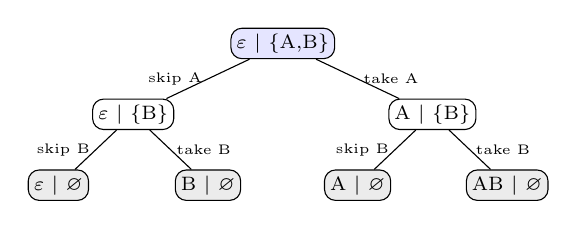
\begin{tikzpicture}[
    level distance=0.90cm,
    level 1/.style={sibling distance=3.8cm},
    level 2/.style={sibling distance=1.9cm},
    every node/.style={draw, rounded corners, font=\scriptsize, inner sep=2pt},
    edge from parent/.style={draw, thin}
  ]
  \node[fill=blue!10] {$\varepsilon$ $|$ $\{$A,B$\}$}
    child { node {$\varepsilon$ $|$ $\{$B$\}$}
      child { node[fill=gray!15] {$\varepsilon$ $|$ $\varnothing$}
        edge from parent node[draw=none, left, font=\tiny] {skip B} }
      child { node[fill=gray!15] {B $|$ $\varnothing$}
        edge from parent node[draw=none, right, font=\tiny] {take B} }
      edge from parent node[draw=none, left, font=\tiny] {skip A}
    }
    child { node {A $|$ $\{$B$\}$}
      child { node[fill=gray!15] {A $|$ $\varnothing$}
        edge from parent node[draw=none, left, font=\tiny] {skip B} }
      child { node[fill=gray!15] {AB $|$ $\varnothing$}
        edge from parent node[draw=none, right, font=\tiny] {take B} }
      edge from parent node[draw=none, right, font=\tiny] {take A}
    };
  \end{tikzpicture}
  \end{center}
  \smallskip
  $A$ are $2^n$ subșiruri, fiecare verificat în $O(n + m)$
  $\Rightarrow$ complexitate totală $O(2^n \cdot (n + m))$, exponențial.
\end{frame}

\begin{frame}{Starea DP și recurența}
  \begin{block}{Stare}
    $dp[i][j] = $ lungimea SCM dintre $A[1..i]$ și $B[1..j]$
  \end{block}
  \begin{block}{Recurență}
    \[
      dp[i][j] = \begin{cases}
        dp[i-1][j-1] + 1 & \text{dacă } A[i] = B[j] \\
        \max\bigl(dp[i-1][j],\; dp[i][j-1]\bigr) & \text{altfel}
      \end{cases}
    \]
    \textbf{Bază:} $dp[i][0] = dp[0][j] = 0$
  \end{block}
  \smallskip
  \textbf{Intuiție:}
  \begin{itemize}\itemsep2pt
    \item $A[i] = B[j]$: ambele caractere fac parte din SCM $\Rightarrow$ extindem cu $+1$
      față de $dp[i-1][j-1]$
    \item $A[i] \neq B[j]$: renunțăm la $A[i]$ sau la $B[j]$, luăm maximul
  \end{itemize}
  \textbf{Complexitate:} $O(n \cdot m)$ timp și spațiu.
\end{frame}

\begin{frame}{Ilustrare \textemdash{} cele două cazuri}
  Exemplu: $A = \texttt{ABCD}$, $B = \texttt{ABDC}$ (celulele $dp[2][2]$ și $dp[2][3]$).
  \begin{columns}[c]
    \column{0.48\textwidth}
    \begin{block}{Cazul 1: $A[i] = B[j]$}
      $i{=}2$, $j{=}2$: B $=$ B\\
      $dp[2][2] = dp[1][1] + 1 = \mathbf{2}$
    \end{block}
    \begin{center}
    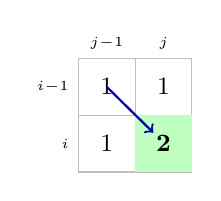
\begin{tikzpicture}
      \draw[step=0.72cm, gray!50] (0,0) grid (1.44,1.44);
      \fill[green!25] (0.72,0) rectangle (1.44,0.72);
      \node[font=\small] at (0.36,1.08) {1};
      \node[font=\small] at (1.08,1.08) {1};
      \node[font=\small] at (0.36,0.36) {1};
      \node[font=\small\bfseries] at (1.08,0.36) {2};
      \draw[->, thick, blue!70!black] (0.36,1.08) -- (0.95,0.50);
      \node[font=\tiny, above] at (0.36,1.44) {$j{-}1$};
      \node[font=\tiny, above] at (1.08,1.44) {$j$};
      \node[font=\tiny, left]  at (0,1.08) {$i{-}1$};
      \node[font=\tiny, left]  at (0,0.36) {$i$};
    \end{tikzpicture}
    \end{center}

    \column{0.48\textwidth}
    \begin{block}{Cazul 2: $A[i] \neq B[j]$}
      $i{=}2$, $j{=}3$: B $\neq$ D\\
      $dp[2][3] = \max(dp[1][3], dp[2][2]) = \mathbf{2}$
    \end{block}
    \begin{center}
    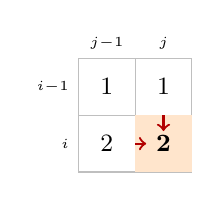
\begin{tikzpicture}
      \draw[step=0.72cm, gray!50] (0,0) grid (1.44,1.44);
      \fill[orange!20] (0.72,0) rectangle (1.44,0.72);
      \node[font=\small] at (0.36,1.08) {1};
      \node[font=\small] at (1.08,1.08) {1};
      \node[font=\small] at (0.36,0.36) {2};
      \node[font=\small\bfseries] at (1.08,0.36) {2};
      \draw[->, thick, red!70!black] (1.08,0.72) -- (1.08,0.52);
      \draw[->, thick, red!70!black] (0.72,0.36) -- (0.86,0.36);
      \node[font=\tiny, above] at (0.36,1.44) {$j{-}1$};
      \node[font=\tiny, above] at (1.08,1.44) {$j$};
      \node[font=\tiny, left]  at (0,1.08) {$i{-}1$};
      \node[font=\tiny, left]  at (0,0.36) {$i$};
    \end{tikzpicture}
    \end{center}
  \end{columns}
\end{frame}

\begin{frame}{Exemplu pas cu pas}
  $A = \texttt{ABCD}$, $B = \texttt{ABDC}$
  \begin{center}
  {\small
  \begin{tabular}{c|ccccc}
    \toprule
    $dp$ & $\varnothing$ & \texttt{A} & \texttt{B} & \texttt{D} & \texttt{C} \\
    \midrule
    $\varnothing$ & 0 & 0 & 0 & 0 & 0 \\
    \texttt{A}    & 0 & \textbf{1} & 1 & 1 & 1 \\
    \texttt{B}    & 0 & 1 & \textbf{2} & 2 & 2 \\
    \texttt{C}    & 0 & 1 & 2 & 2 & \textbf{3} \\
    \texttt{D}    & 0 & 1 & 2 & \textbf{3} & 3 \\
    \bottomrule
  \end{tabular}}
  \end{center}
  \smallskip
  \textbf{Celule bold} = potrivire $A[i]=B[j]$, extindem diagonal ($+1$).\\
  Celulele fără potrivire = maximul din stânga sau de sus.
  \smallskip
  Răspuns: $dp[4][4] = 3$ \textemdash{} SCM poate fi \texttt{ABC} sau \texttt{ABD}.
\end{frame}

\begin{frame}[fragile]{Implementare}
  \begin{lstlisting}
const int nmax = 1000;
int dp[nmax + 1][nmax + 1];
char A[nmax + 1], B[nmax + 1];

// n, m, A[], B[] citite anterior (indexate de la 1)
for (int i = 1; i <= n; i++) {
    for (int j = 1; j <= m; j++) {
        if (A[i] == B[j]) {
            dp[i][j] = dp[i - 1][j - 1] + 1;
        } else {
            dp[i][j] = max(dp[i - 1][j], dp[i][j - 1]);
        }
    }
}
// Raspuns: dp[n][m]
  \end{lstlisting}
  \textbf{Obs:} $dp[i][0]$ și $dp[0][j]$ sunt implicit $0$ (variabile globale).
\end{frame}

\begin{frame}[fragile]{Reconstrucția soluției}
  \textbf{Idee:} parcurgem $dp$ înapoi de la $(n, m)$ spre $(0, 0)$:
  \begin{itemize}\itemsep1pt
    \item $A[i]=B[j]$: caracterul face parte din SCM $\Rightarrow$ mergem diagonal
    \item Altfel: mergem spre celula mai mare (sus sau stânga)
  \end{itemize}
  \begin{lstlisting}
string scm = "";
int i = n, j = m;
while (i > 0 && j > 0) {
    if (A[i] == B[j]) {
        scm += A[i];
        i--;
        j--;
    } else if (dp[i - 1][j] >= dp[i][j - 1]) {
        i--;
    } else {
        j--;
    }
}
reverse(scm.begin(), scm.end());
  \end{lstlisting}
\end{frame}

\begin{frame}[fragile]{Reconstrucția \textemdash{} traseu în tabel}
  $A = \texttt{ABCD}$, $B = \texttt{ABDC}$: pornim din $dp[4][4]$, mergem înapoi.
  \begin{columns}[c]
    \column{0.52\textwidth}
    \begin{center}
    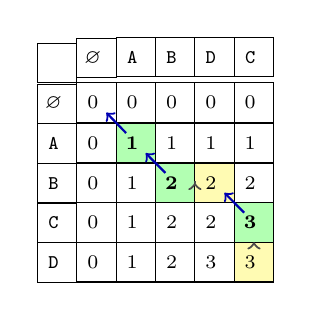
\begin{tikzpicture}
    \matrix (T) [
      matrix of nodes,
      nodes={draw, minimum size=0.50cm, font=\scriptsize,
             inner sep=0pt, outer sep=0pt, align=center},
      row sep=-\pgflinewidth,
      column sep=-\pgflinewidth
    ] {
      {} & $\varnothing$ & \texttt{A} & \texttt{B} & \texttt{D} & \texttt{C} \\
      $\varnothing$ & 0 & 0 & 0 & 0 & 0 \\
      \texttt{A} & 0 & |[fill=green!30]| \textbf{1} & 1 & 1 & 1 \\
      \texttt{B} & 0 & 1 & |[fill=green!30]| \textbf{2} & |[fill=yellow!30]| 2 & 2 \\
      \texttt{C} & 0 & 1 & 2 & 2 & |[fill=green!30]| \textbf{3} \\
      \texttt{D} & 0 & 1 & 2 & 3 & |[fill=yellow!30]| 3 \\
    };
    % (4,4)->(3,4): up
    \draw[->, thick, black!70] (T-6-6.north) -- (T-5-6.south);
    % (3,4)->(2,3): diagonal
    \draw[->, thick, blue!70!black]
      ($(T-5-6.center)!0.25!(T-4-5.center)$) --
      ($(T-5-6.center)!0.75!(T-4-5.center)$);
    % (2,3)->(2,2): left
    \draw[->, thick, black!70] (T-4-5.west) -- (T-4-4.east);
    % (2,2)->(1,1): diagonal
    \draw[->, thick, blue!70!black]
      ($(T-4-4.center)!0.25!(T-3-3.center)$) --
      ($(T-4-4.center)!0.75!(T-3-3.center)$);
    % (1,1)->(0,0): diagonal (stop)
    \draw[->, thick, blue!70!black]
      ($(T-3-3.center)!0.25!(T-2-2.center)$) --
      ($(T-3-3.center)!0.75!(T-2-2.center)$);
    \end{tikzpicture}
    \end{center}

    \column{0.44\textwidth}
    {\footnotesize
    \begin{enumerate}\itemsep3pt
      \item $(4,4)$: D$\neq$C\\$\uparrow$ sus la $(3,4)$
      \item $(3,4)$: C$=$C \checkmark\\$\nwarrow$ diagonal la $(2,3)$
      \item $(2,3)$: B$\neq$D\\$\leftarrow$ stânga la $(2,2)$
      \item $(2,2)$: B$=$B \checkmark\\$\nwarrow$ diagonal la $(1,1)$
      \item $(1,1)$: A$=$A \checkmark\\$\nwarrow$ diagonal la $(0,0)$
    \end{enumerate}
    \smallskip
    scm $= $ CBA $\xrightarrow{\text{reverse}}$ \textbf{ABC}}
  \end{columns}
  \vspace{2pt}
  {\scriptsize
  \textcolor{green!50!black}{$\blacksquare$} potrivire\quad
  \textcolor{yellow!60!black}{$\blacksquare$} fără potrivire\quad
  \textcolor{blue!70!black}{$\nearrow$} diagonal\quad
  \textcolor{gray!70}{$\rightarrow$/$\uparrow$} stânga/sus}
\end{frame}

%% ============================================================
\section{Problema Rucsacului}
%% ============================================================

\begin{frame}{Rucsac fractionar}
  \begin{block}{Variantă}
    Putem lua \textbf{fracțiuni} din obiecte: fracțiunea $f_i \in [0,1]$ din obiectul $i$
    adaugă greutate $f_i \cdot g_i$ și valoare $f_i \cdot v_i$.
  \end{block}
  \textbf{Greedy:} sortăm descrescător după $v_i/g_i$ și luăm cât putem din fiecare.
  \begin{center}
  {\small\begin{tabular}{lcccc}
    \toprule
    Obiect & $g_i$ & $v_i$ & $v_i/g_i$ & Luat \\
    \midrule
    A & 10 & 60 & 6.0 & tot (10 kg) \\
    B & 20 & 100 & 5.0 & tot (20 kg) \\
    C & 30 & 120 & 4.0 & $\frac{2}{3}$ (20 kg din 30) \\
    \bottomrule
  \end{tabular}}
  \end{center}
  $W = 50$: valoare $= 60 + 100 + 80 = \mathbf{240}$. \textbf{Complexitate:} $O(n \log n)$.
  \smallskip
  \textbf{De ce greedy nu merge pentru 0/1:} nu putem lua fracțiuni \textemdash{} fiecare
  obiect e întreg sau absent. Un obiect greu cu raport bun poate „bloca" combinații mai valoroase.
\end{frame}

\begin{frame}{Rucsac 0/1 \textemdash{} backtracking}
  \begin{block}{Problemă}
    Se dau $n$ obiecte cu greutăți $g_i$ și valori $v_i$, capacitate $W$.
    Fiecare obiect poate fi luat \textbf{cel mult o dată}. Maximizați valoarea.
  \end{block}
  \smallskip
  \textbf{Backtracking:} la fiecare obiect decidem \textit{luăm} sau \textit{nu luăm}.
  \begin{itemize}\itemsep2pt
    \item $2^n$ submulțimi posibile $\Rightarrow$ complexitate $O(2^n)$, inacceptabil
    \item Aceeași stare $(i, w)$ se recalculează exponențial de multe ori
  \end{itemize}
  \smallskip
  \textbf{Soluție DP:} definim $dp[i][w]$ = valoarea maximă folosind primele $i$ obiecte
  cu capacitate $w$. Calculăm fiecare stare \textbf{o singură dată} $\Rightarrow O(n \cdot W)$.
\end{frame}

\begin{frame}{Rucsac 0/1 \textemdash{} starea DP și recurența}
  \begin{block}{Stare}
    $dp[i][w] = $ valoarea maximă folosind primele $i$ obiecte cu capacitate $w$
  \end{block}
  \begin{block}{Recurență}
    \[
      dp[i][w] = \begin{cases}
        dp[i-1][w] & \text{dacă } g_i > w\;\text{(nu încape)} \\
        \max\!\bigl(dp[i-1][w],\; dp[i-1][w-g_i]+v_i\bigr) & \text{altfel}
      \end{cases}
    \]
    \textbf{Bază:} $dp[0][w] = 0$ pentru orice $w$. \quad \textbf{Răspuns:} $dp[n][W]$.
  \end{block}
  \smallskip
  \textbf{Intuiție:}
  \begin{itemize}\itemsep1pt
    \item \textbf{Nu luăm obiectul $i$:} $dp[i-1][w]$ \textemdash{} aceeași capacitate, fără obiectul $i$
    \item \textbf{Luăm obiectul $i$} (dacă $g_i \le w$): $dp[i-1][w-g_i] + v_i$
  \end{itemize}
  \textbf{Complexitate:} $O(n \cdot W)$ timp, $O(n \cdot W)$ spațiu.
\end{frame}

\begin{frame}[fragile]{Rucsac 0/1 \textemdash{} implementare 2D}
  \begin{lstlisting}
const int nmax = 5000;
const int wmax = 10000;
int g[nmax + 1], v[nmax + 1];
int dp[nmax + 1][wmax + 1];

// n, W, g[], v[] citite (indexate de la 1)
for (int i = 1; i <= n; i++) {
    for (int w = 0; w <= W; w++) {
        dp[i][w] = dp[i - 1][w];
        if (g[i] <= w) {
            dp[i][w] = max(dp[i][w], dp[i - 1][w - g[i]] + v[i]);
        }
    }
}
// Raspuns: dp[n][W]
  \end{lstlisting}
  \textbf{Obs:} pentru $n = 5000$, $W = 10000$ rezultă $5 \cdot 10^7$ celule \textemdash{}
  adesea prea mult ca memorie. Folosim optimizarea 1D.
\end{frame}

\begin{frame}[fragile]{Rucsac 0/1 \textemdash{} optimizare memorie $O(W)$}
  La calculul rândului $i$ avem nevoie \textbf{doar de rândul $i-1$}
  $\Rightarrow$ reducem la un singur vector, parcurgând \textbf{de la dreapta la stânga}:
  \begin{lstlisting}
const int wmax = 10000;
int dp[wmax + 1];

for (int i = 1; i <= n; i++) {
    for (int w = W; w >= g[i]; w--) {
        dp[w] = max(dp[w], dp[w - g[i]] + v[i]);
    }
}
// Raspuns: dp[W]
  \end{lstlisting}
  \begin{block}{De ce dreapta la stânga?}
    La pasul $i$, $dp[w - g_i]$ trebuie să fie valoarea \textbf{înainte} de procesarea
    obiectului $i$ (rândul $i-1$). Parcurgând descrescător, $dp[w - g_i]$ nu e încă
    suprascris cu valoarea de la pasul $i$, deci fiecare obiect e luat \textbf{cel mult o dată}.
  \end{block}
\end{frame}

\begin{frame}{Rucsac unbounded \textemdash{} definiție și recurență}
  \begin{block}{Variantă}
    Fiecare obiect poate fi luat de \textbf{oricâte ori} (copii nelimitate).
  \end{block}
  \smallskip
  \textbf{Recurență 2D:}
  \[
    dp[i][w] = \begin{cases}
      dp[i-1][w] & \text{dacă } g_i > w \\
      \max\!\bigl(dp[i-1][w],\; \textcolor{blue}{dp[i]}[w-g_i]+v_i\bigr) & \text{altfel}
    \end{cases}
  \]
  Diferența față de 0/1: folosim $dp[\textcolor{blue}{i}][w-g_i]$ (același rând $i$, nu $i-1$)
  \textemdash{} aceasta permite refolosirea obiectului $i$ în aceeași selecție.
  \smallskip
  \textbf{Consecință pentru 1D:} parcurgem $w$ \textbf{de la stânga la dreapta} (crescător),
  astfel $dp[w - g_i]$ e deja actualizat pentru obiectul $i$ când ajungem la $w$.
  \[
    dp[w] = \max_{i:\,g_i \le w}\bigl(dp[w - g_i] + v_i\bigr)
  \]
  \textbf{Complexitate:} $O(n \cdot W)$ timp, $O(W)$ spațiu (1D direct).
\end{frame}

\begin{frame}[fragile]{Rucsac unbounded \textemdash{} implementare $O(W)$}
  \begin{lstlisting}
const int wmax = 10000;
int dp[wmax + 1];  // dp[0] = 0

for (int i = 1; i <= n; i++) {
    for (int w = g[i]; w <= W; w++) {  // stanga la dreapta!
        dp[w] = max(dp[w], dp[w - g[i]] + v[i]);
    }
}
// Raspuns: dp[W]
  \end{lstlisting}
  \smallskip
  \textbf{Comparație directă cu 0/1:}
  \begin{center}
  {\small\begin{tabular}{lll}
    \toprule
    Variantă & Direcție buclă $w$ & De ce? \\
    \midrule
    0/1 & $W \to g_i$ (descrescător) & $dp[w-g_i]$ să nu fie încă actualizat \\
    Unbounded & $g_i \to W$ (crescător) & $dp[w-g_i]$ să fie deja actualizat \\
    \bottomrule
  \end{tabular}}
  \end{center}
\end{frame}

\begin{frame}{Subset Sum \textemdash{} definiție}
  \begin{block}{Problemă}
    Date $n$ numere întregi $a[1..n]$, există o submulțime cu suma \textbf{exact} $S$?
  \end{block}
  \smallskip
  \textbf{Legătura cu rucsacul 0/1:} Subset Sum este un caz particular
  unde $g_i = v_i = a[i]$ și vrem să atingem valoarea exactă $S$.
  \smallskip
  \textbf{Stare:} $dp[w] = $ \texttt{true} dacă există o submulțime cu suma $w$.
  \[
    dp[w] = dp[w] \;\mathbf{OR}\; dp[w - a[i]]
  \]
  \textbf{Bază:} $dp[0] = \text{true}$; $dp[w] = \text{false}$ pentru $w > 0$.
  \textbf{Răspuns:} $dp[S]$.
  \smallskip
  \textbf{Variante frecvente:}
  \begin{itemize}\itemsep1pt
    \item \textbf{Număr de submulțimi} cu suma $S$: \texttt{bool} $\to$ \texttt{long long}, OR $\to$ $+=$
    \item \textbf{Valoare maximă} $\le S$: cel mai mare $w \le S$ cu $dp[w] = \text{true}$
    \item \textbf{Toate sumele posibile}: $dp[w]$ rămâne \texttt{true} pentru toate sumele atinse
  \end{itemize}
\end{frame}

\begin{frame}[fragile]{Subset Sum \textemdash{} implementare}
  \begin{lstlisting}
const int smax = 100000;
bool dp[smax + 1];

dp[0] = true;
for (int i = 1; i <= n; i++) {
    for (int w = S; w >= a[i]; w--) {  // invers (0/1, fiecare o singura data)
        dp[w] |= dp[w - a[i]];
    }
}
// Raspuns: dp[S]
  \end{lstlisting}
  \smallskip
  \textbf{Obs:} dacă fiecare element poate fi folosit de mai multe ori (Subset Sum unbounded):
  \begin{lstlisting}
for (int i = 1; i <= n; i++) {
    for (int w = a[i]; w <= S; w++) {  // crescator
        dp[w] |= dp[w - a[i]];
    }
}
  \end{lstlisting}
  \textbf{Complexitate:} $O(n \cdot S)$ timp, $O(S)$ spațiu.
\end{frame}

\begin{frame}[fragile]{Optimizări}
  \begin{block}{Bitset \textemdash{} Subset Sum în $O(nS/64)$}
    Reprezentăm $dp$ ca \texttt{bitset}: bitul $w$ = 1 dacă suma $w$ e posibilă.
    Tranziția $dp[w] \mathrel{|}= dp[w - a[i]]$ devine un \textbf{shift} și \textbf{OR}
    pe tot bitset-ul simultan:
  \end{block}
  \begin{lstlisting}
bitset<100001> dp;
dp[0] = 1;
for (int i = 1; i <= n; i++) {
    dp |= (dp << a[i]);  // O(S/64) per element
}
// Raspuns: dp[S]
  \end{lstlisting}
  \begin{block}{Grupare pe puteri de 2 \textemdash{} obiecte egale în cantitate mare}
    Dacă avem $k$ copii ale unui obiect cu greutate $g$, în loc de $k$ tranziții identice
    le grupăm în $\lceil \log_2 k \rceil + 1$ \textbf{pachete}: $1,\; 2,\; 4,\;\ldots,\;\text{rest}$.
    Fiecare pachet e tratat ca un obiect 0/1 separat.
    Numărul de tranziții scade de la $O(k)$ la $O(\log k)$ per grup.
  \end{block}
\end{frame}

%% ============================================================
\section{Recapitulare}
%% ============================================================

\begin{frame}{Probleme de antrenament}
  \begin{enumerate}\itemsep2pt\normalsize
    \item \href{https://www.infoarena.ro/problema/rucsac}{\textbf{rucsac}}
          \textcolor{gray}{(infoarena)} \textemdash{} 0/1 Knapsack clasic
    \item \href{https://www.pbinfo.ro/probleme/819/ghiozdan}{\textbf{ghiozdan}}
          \textcolor{gray}{(pbinfo \#819)} \textemdash{} 0/1 Knapsack
    \item \href{https://cses.fi/problemset/task/1158}{\textbf{Book Shop}}
          \textcolor{gray}{(CSES \#1158)} \textemdash{} 0/1 Knapsack
    \item \href{https://cses.fi/problemset/task/1634}{\textbf{Minimizing Coins}}
          \textcolor{gray}{(CSES \#1634)} \textemdash{} Unbounded \textemdash{} nr. minim de monede pentru suma $X$
    \item \href{https://cses.fi/problemset/task/1636}{\textbf{Coin Combinations II}}
          \textcolor{gray}{(CSES \#1636)} \textemdash{} Unbounded \textemdash{} câte moduri neordonate
    \item \href{https://cses.fi/problemset/task/1745}{\textbf{Money Sums}}
          \textcolor{gray}{(CSES \#1745)} \textemdash{} Subset Sum \textemdash{} toate sumele posibile
    \item \href{https://codeforces.com/problemset/problem/545/C}{\textbf{Woodcutters}}
          \textcolor{gray}{(CF \#545C)} \textemdash{} SCM cu condiții suplimentare
  \end{enumerate}
\end{frame}

\begin{frame}{Resurse}
  \begin{enumerate}\itemsep2pt\normalsize
    \item \href{https://www.pbinfo.ro/articole/22/cel-mai-lung-subsir-comun}{\textbf{pbinfo}}
          \textemdash{} Cel mai lung subșir comun (în română)
    \item \href{https://www.pbinfo.ro/articole/23/problema-rucsacului}{\textbf{pbinfo}}
          \textemdash{} Problema Rucsacului (în română)
    \item \href{https://www.geeksforgeeks.org/dsa/0-1-knapsack-problem-dp-10/}{\textbf{GeeksforGeeks}}
          \textemdash{} 0/1 Knapsack \textemdash{} recursiv, memo, tabelar, $O(W)$
    \item \href{https://usaco.guide/gold/knapsack}{\textbf{USACO Guide}}
          \textemdash{} Knapsack DP \textemdash{} 0/1, Subset Sum, probleme Gold
    \item \href{https://cp-algorithms.com/dynamic_programming/knapsack.html}{\textbf{CP-Algorithms}}
          \textemdash{} Knapsack Problems \textemdash{} toate variantele
    \item \href{https://codeforces.com/blog/entry/98663}{\textbf{Codeforces blog \#98663}}
          \textemdash{} Knapsack, Subset Sum \textemdash{} optimizări avansate cu bitset
  \end{enumerate}
\end{frame}

\end{document}
